\chapter{Estabilidad asintótica}

\section{Motivación. Ecuación test de Dahlquist}

Consideremos el siguiente problema de Cauchy:
\begin{align*}
    \left\{ \begin{array}{lcc}
                y' = \lambda y, \ \ \text{Re}(\lambda) < 0 \\
                y(0) = y_0                                 \\
            \end{array}
    \right.
\end{align*}
La única solución de dicho problema es $y(t) = y_0e^{\lambda t}$ y todas las soluciones de la ecuación $y' = \lambda y$ verifican que:
\begin{align*}
    \lim_{t \to \infty} y(t) = 0.
\end{align*}
Apliquemos el método de Euler a este problema. Tenemos entonces el método
\begin{align*}
    y_{k+1} & = y_k + hf(t_k,y_k)                         \\
            & = y_k + h\lambda y_k, \ \ k = 0,1,2,\ldots.
\end{align*}
¿Para qué valores de $h$ ocurre que $\lim_{t \to \infty} y_k = 0$?
\begin{align*}
    y_0 & = y_0                                   \\
    y_1 & = y_0(1+ h\lambda)                      \\
    y_2 & = y_1(1+ h\lambda) = y_0(1+ h\lambda)^2 \\
        & \vdots                                  \\
    y_k & = y_0(1+h\lambda)^k
\end{align*}
Entonces
\begin{align*}
    \lim_{k \to \infty} y_k = 0 \Longleftrightarrow |1+ h\lambda|^k < 1 \Longleftrightarrow h < -\frac{2}{\lambda}
\end{align*}
Si $0 < 1 +h\lambda < 1$ la convergencia es monótona y esto ocurre si y solo si $h < -1/\lambda$. Distingamos los distintos casos:
\begin{enumerate}
    \item Si $h \in \left(0,-\frac{1}{\lambda}\right)$ entonces $y_k \xrightarrow[k \to \infty]{} 0$ de forma monótona. Si tomamos $\lambda = -5$:
          \begin{align*}
              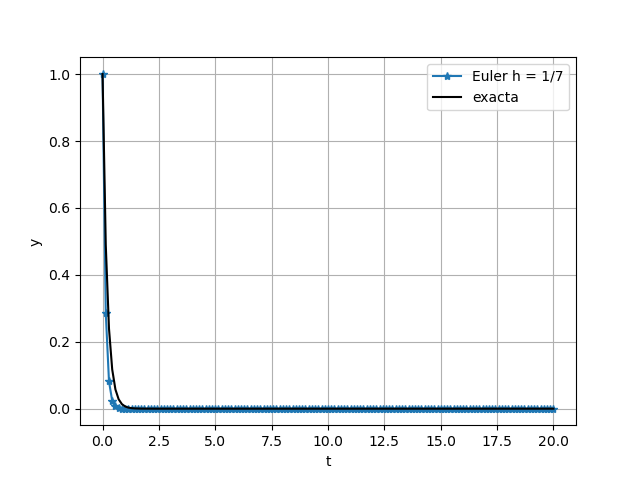
\includegraphics[width=0.5\textwidth]{imagenes/Caso_1.png}
          \end{align*}
    \item Si $h = -\frac{1}{\lambda}$. Si tomamos $\lambda = -5$:
          \begin{align*}
              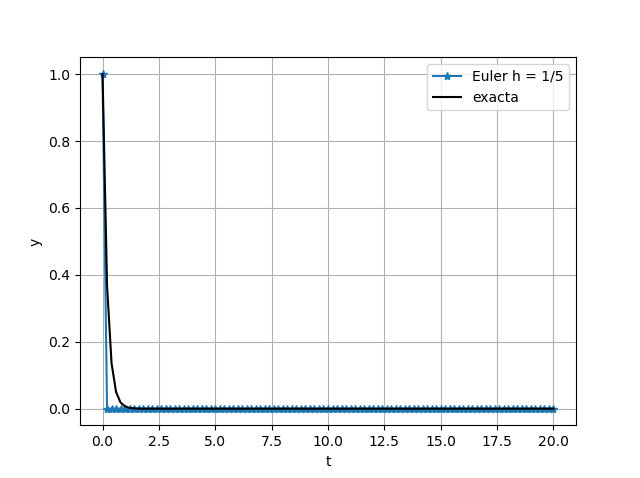
\includegraphics[width=0.5\textwidth]{imagenes/Caso_2.png}
          \end{align*}
    \item Si $h \in \left(-\frac{1}{\lambda},-\frac{2}{\lambda}\right)$. Si tomamos $\lambda = -5$:
          \begin{align*}
              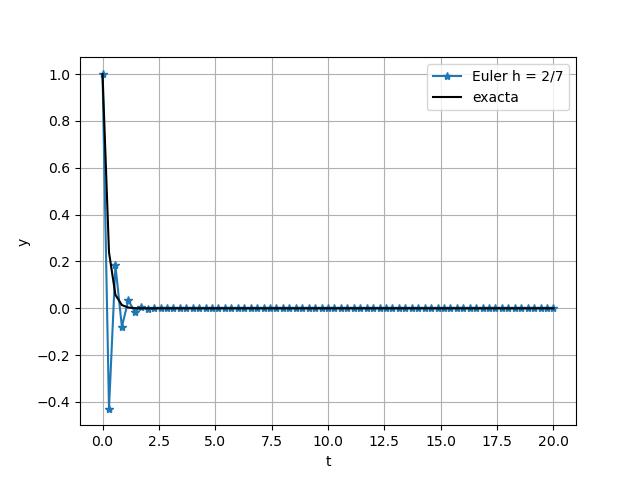
\includegraphics[width=0.5\textwidth]{imagenes/Caso_3.png}
          \end{align*}
    \item Si $h = -\frac{2}{\lambda}$. Si tomamos $\lambda = -5$:
          \begin{align*}
              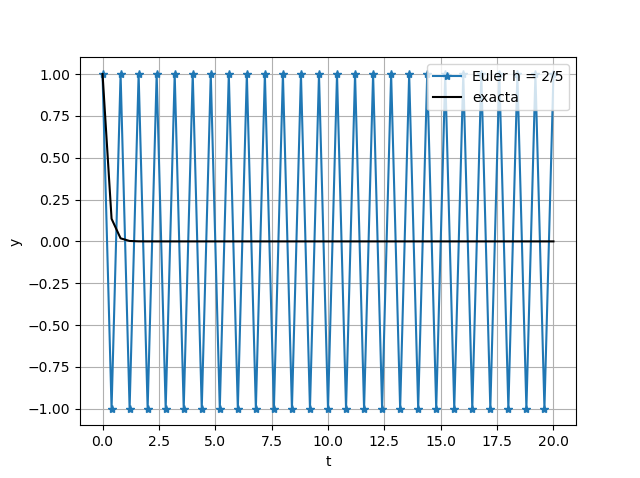
\includegraphics[width=0.5\textwidth]{imagenes/Caso_4.png}
          \end{align*}
    \item Si $h > -\frac{2}{\lambda}$ entonces $|y_k| \xrightarrow[k \to \infty]{} \infty$. Si tomamos $\lambda = -5$:
          \begin{align*}
              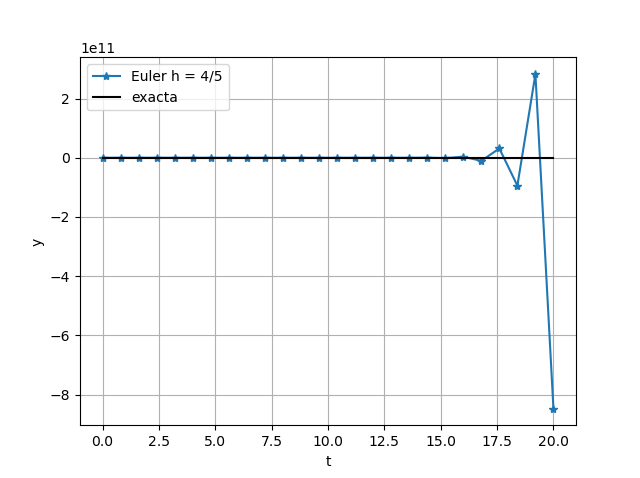
\includegraphics[width=0.5\textwidth]{imagenes/Caso_5.png}
          \end{align*}
\end{enumerate}

\begin{defi}
    A la función $R(\hat{h}) = 1+ \hat{h}$, siendo $\hat{h} = h\lambda$, se le denomina función de estabilidad absoluta del método de Euler. Si $\text{Re}(\lambda) < 0$, se denomina intervalo de estabilidad absoluta a $I_A = \{ \hat{h} : |R(\hat{h})| < 1\}$.
\end{defi}

\begin{ejemplo}
    Encontrar la función de estabilidad absoluta y el intervalo de estabilidad absoluta para el método de Euler implícito aplicandolo al problema:
    \begin{align*}
        \left\{ \begin{array}{lcc}
                    y' = \lambda y, \ \ \text{Re}(\lambda) < 0 \\
                    y(0) = y_0                                 \\
                \end{array}
        \right.
    \end{align*}
    Tenemos que:
    \begin{align*}
        y_{k+1} & = y_k + hf(t_{k+1},y_{k+1}) \\
                & = y_k + h\lambda y_{k+1}
    \end{align*}
    De donde deducimos que $y_{k+1} = \frac{1}{1-\hat{h}}y_k$, siendo $\hat{h} = h\lambda$. Así
    \begin{align*}
        |R(\hat{h})| < 1 \Longleftrightarrow \left| \frac{1}{1-\hat{h}} \right| < 1 \Longleftrightarrow \hat{h} < 0 \Longrightarrow I_A = (-\infty,0)
    \end{align*}
    Si $\lambda \in \mathbb{C}$ y $\text{Re}(\lambda) < 0$, entonces las soluciones de la ecuación del problema se pueden expresar como
    \begin{align*}
        y(t) = y_0 e^{\lambda t} = y_0 e^{\text{Re}(\lambda)t}[\cos(\text{Im}(\lambda)t) + i\sen(\text{Im}(\lambda)t)].
    \end{align*}
    Como $\cos(\text{Im}(\lambda)t) + i\sen(\text{Im}(\lambda)t)$ está acotada, entonces $\lim_{t \to \infty} y(t) = 0$ para toda solución de la ecuación. Aplicando el método de Euler  llegamos a que
    \begin{align*}
        y_k = (1 + h\lambda)^ky_0, \ \ k = 0,1,2,\ldots.
    \end{align*}
    \begin{align*}
        \lim_{k \to \infty} y_k = 0 \Longleftrightarrow |1+ h\lambda|^k < 1 \Longleftrightarrow |1 + \hat{h}| < 1 \Longleftrightarrow \hat{h} \in \Delta(-1,1).
    \end{align*}
    A $\{ \hat{h} \in \mathbb{C} : |R(\hat{h})| < 1\}$ se le denomina dominio de estabilidad.

    Si aplicamos Euler implícito llegamos a que
    \begin{align*}
        |R(\hat{h})| < 1 \Longleftrightarrow \left| \frac{1}{1-\hat{h}} \right| < 1 \Longleftrightarrow  1 < |1 -\hat{h}| \Longleftrightarrow |\hat{h} -1| > 1.
    \end{align*}
    Así, la región de estabilidad es el el exterior del disco $\Delta(1,1)$.
    \begin{figure}[H]
        \centering
        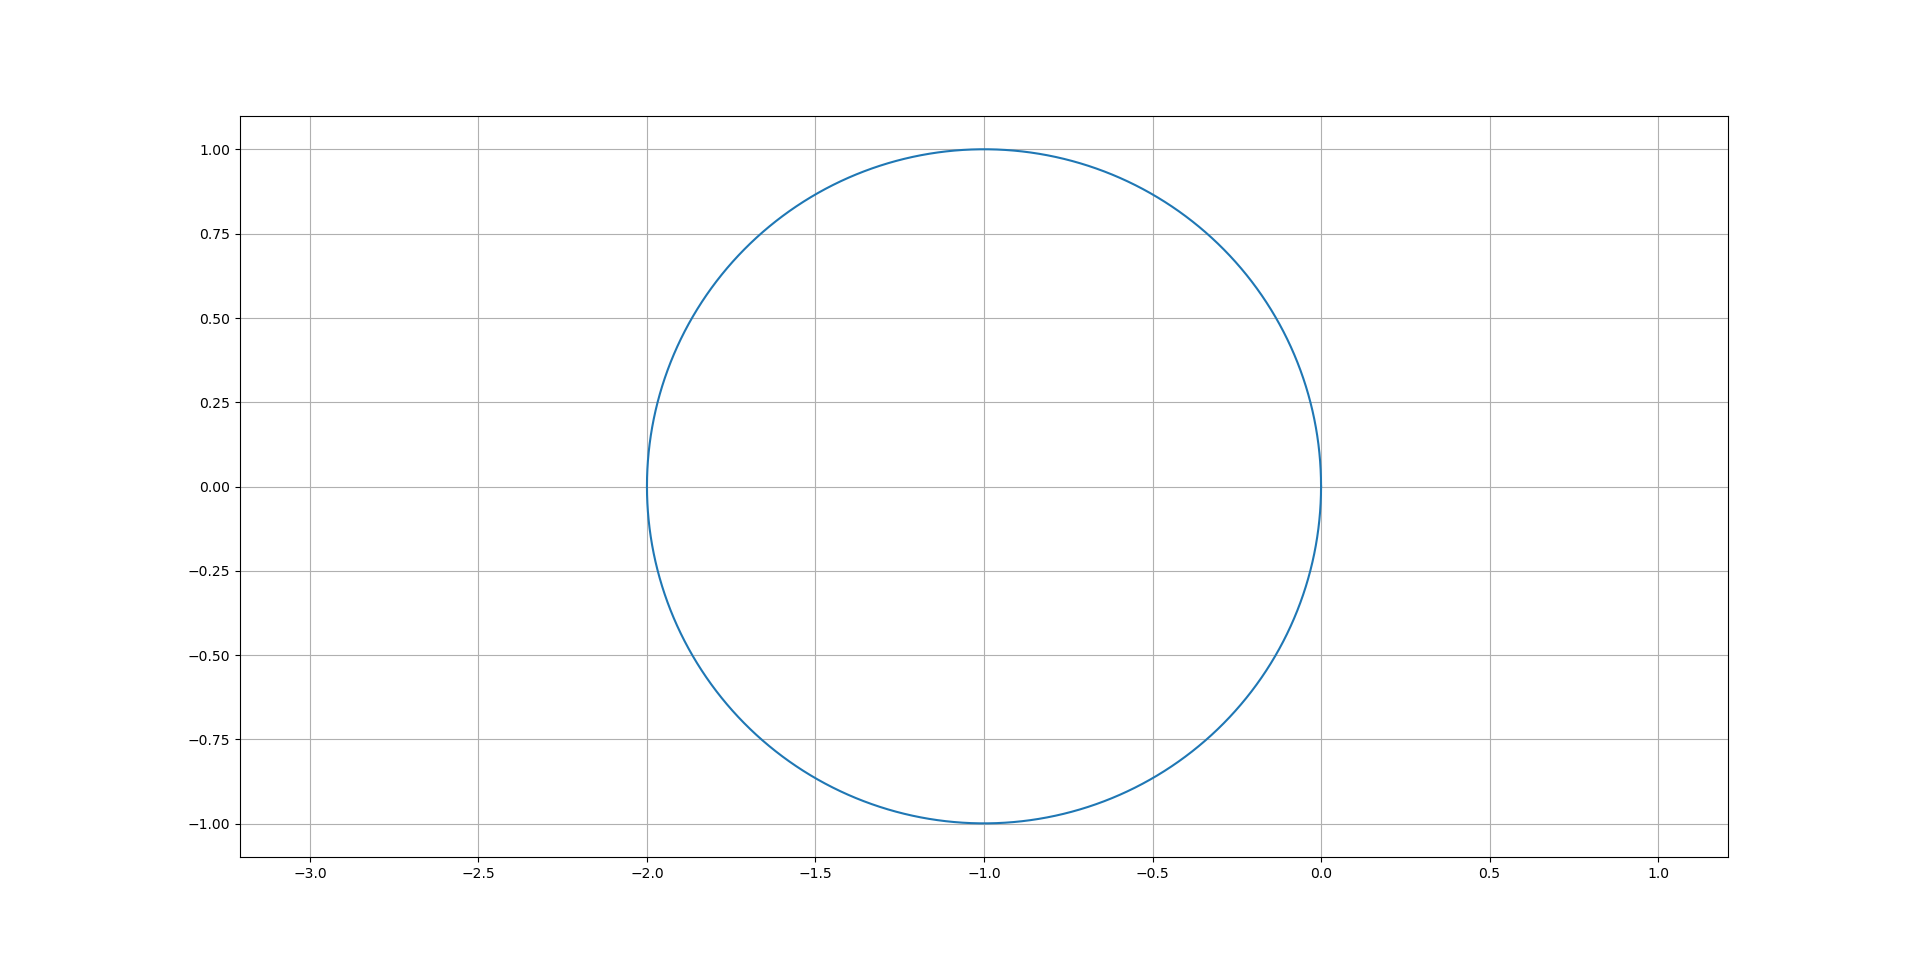
\includegraphics[width=1\textwidth]{imagenes/Euler_implicito.png}
        \caption*{Frontera del dominio de estabilidad del método Euler implícito.}
    \end{figure}
\end{ejemplo}

Supongamos ahora que tenemos un sistema lineal de ecuaciones diferenciales
\begin{align*}
    \left\{ \begin{array}{lcc}
                \overrightarrow{y}' = M\overrightarrow{y} \\
                \overrightarrow{y}(0) = \overrightarrow{y_0}
            \end{array}
    \right., \ \ \overrightarrow{y} = \begin{bmatrix}
                                          y_1    \\
                                          \vdots \\
                                          y_N
                                      \end{bmatrix}, \ \ M = \begin{bmatrix}
                                                                 m_{11} & \cdots & m_{1N} \\
                                                                 \vdots & \ddots & \vdots \\
                                                                 m_{N1} & \cdots & m_{NN}
                                                             \end{bmatrix}
\end{align*}
Supongamos que $M$ es diagonalizable, con autovalores $\lambda_1,\ldots,\lambda_N \in \mathbb{C}$. ¿Bajo qué condiciones se puede asegurar que $\lim_{t \to \infty} \overrightarrow{y}(t) = 0$ para toda solución del sistema?

Como $M$ es diagonalizable, entonces $M = Q\Lambda Q^{-1}$ donde
\begin{align*}
    \Lambda = \begin{bmatrix}
                  \lambda_1 & \cdots & 0         \\
                  \vdots    & \ddots & \vdots    \\
                  0         & \cdots & \lambda_N
              \end{bmatrix}, \ \ \ Q = [R_1 | \cdots | R_N]
\end{align*}
siendo $MR_i = \lambda_iR_i$ para cada $i = 1,\ldots,N$.

Si cambiamos de la base canónica a la base de los autovalores, tenemos que
\begin{align*}
    \overrightarrow{Z}(t)  & = Q^{-1}\overrightarrow{y}(t)                                                                                                 \\
    \overrightarrow{Z}'(t) & = Q^{-1}\overrightarrow{y}'(t) = Q^{-1}M\overrightarrow{y}(t) = Q^{-1}MQ\overrightarrow{Z}(t) = \Lambda \overrightarrow{Z}(t)
\end{align*}
es decir,
\begin{align*}
    \begin{bmatrix}
        Z_1'   \\
        \vdots \\
        Z_N '
    \end{bmatrix} = \begin{bmatrix}
                        \lambda_1 & \cdots & 0         \\
                        \vdots    & \ddots & \vdots    \\
                        0         & \cdots & \lambda_N
                    \end{bmatrix} \cdot \begin{bmatrix}
                                            Z_1    \\
                                            \vdots \\
                                            Z_N
                                        \end{bmatrix} \Longleftrightarrow Z_i' = \lambda _i Z_i, \ \ i = 1,\ldots,N.
\end{align*}
Por tanto, la solución es $Z_i(t) = Z_{i,0}e^{\lambda_i t}$ siendo
\begin{align*}
    \overrightarrow{Z}_0 = Q^{-1}\overrightarrow{y_0} = \begin{bmatrix}
                                                            Z_{1,0} \\
                                                            \vdots  \\
                                                            Z_{N,0}
                                                        \end{bmatrix},
\end{align*}
lo que nos dice que
\begin{align*}
    \overrightarrow{Z}(t) = \begin{bmatrix}
                                Z_{1,0}e^{\lambda_1 t} \\
                                \vdots                 \\
                                Z_{N,0}e^{\lambda_N t}
                            \end{bmatrix}.
\end{align*}
Así, $\overrightarrow{y}(t) = Q\overrightarrow{Z}(t)$, luego $\lim_{t \to \infty} \overrightarrow{y}(t) = 0$ si y solo si los autovalores son complejos con parte real negativa (lo que incluye el caso de que sean reales y negativos).

Si aplicamos el método de Euler:
\begin{align*}
    \overrightarrow{y_{k+1}} & = \overrightarrow{y_k} + hM\overrightarrow{y_k}.
\end{align*}
¿Cuando podemos afirmar que $\lim_{k \to \infty} \overrightarrow{y_k} = 0$?
\begin{align*}
    \overrightarrow{Z_{k+1}} & = Q^{-1}\overrightarrow{y_{k+1}} = Q(\overrightarrow{y_{k}} + hM\overrightarrow{y_K}) = \overrightarrow{Z_k} + h\Lambda\overrightarrow{Z_k} \\
                             & = (I +h\Lambda)\overrightarrow{Z_k}                                                                                                         \\
                             & = \begin{bmatrix}
                                     1 + h\lambda_1 & \cdots & 0            \\
                                     \vdots         & \ddots & \vdots       \\
                                     0              & \cdots & 1+h\lambda_N
                                 \end{bmatrix} \cdot \begin{bmatrix}
                                                         Z_{1,k} \\
                                                         \vdots  \\
                                                         Z_{N,k}
                                                     \end{bmatrix}.
\end{align*}
Así,
\begin{align*}
    \overrightarrow{Z_k} = \begin{bmatrix}
                               (1+h\lambda_1)^kZ_{1,0} \\
                               \vdots                  \\
                               (1+h\lambda_N)^kZ_{N,0}
                           \end{bmatrix}.
\end{align*}
Por tanto, $\lim_{k \to \infty} \overrightarrow{y_k} = 0$ si y solo si $|1+h\lambda_i|< 1 $ para cada $i = 1,\ldots,N$.

\section{Estabilidad absoluta de los métodos RK}
Al igual que antes, consideremos el problema
\begin{align*}
    \left\{ \begin{array}{lcc}
                y' = \lambda y, \ \ \text{Re}(\lambda) < 0 \\
                y(0) = y_0                                 \\
            \end{array}
    \right.
\end{align*}
cuya solución es
\begin{align*}
    y(t) = y_0 e^{\text{Re}(\lambda)t}[\cos(\text{Im}(\lambda)t) + i\sen(\text{Im}(\lambda)t)]
\end{align*}
Apliquemos un método RK con el siguiente tablero de Butcher
\begin{tabular}{c|ccc}
    $c_1$    & $a_{11}$ & $\cdots$ & $a_{1q}$ \\
    $\vdots$ & $\vdots$ & $\ddots$ & $\vdots$ \\
    $c_q$    & $a_{q1}$ & $\cdots$ & $a_{qq}$ \\
    \hline
             & $b_1$    & $\cdots$ & $b_q$
\end{tabular}
Hemos de resolver:
\begin{align*}
    \left. \begin{array}{lcr}    y_k^{(1)} & = y_k + \lambda h \sum_{j=1}^{q} a_{1,j} y_k^{(j)} \\
             y_k^{(2)}          & = y_k + \lambda h \sum_{j=1}^{q} a_{2,j} y_k^{(j)} \\
                                & \vdots                                             \\
             y_k^{(q)}          & = y_k + \lambda h \sum_{j=1}^{q} a_{q,j} y_k^{(j)} \\
             y_{k+1}            & = \lambda h \sum_{i=1}^{q} b_i y_k^{(j)}
           \end{array}
    \right\} \Longleftrightarrow Y = y_k \overrightarrow{e} + \hat{h} AY.
\end{align*}
siendo:
\begin{align*}
    A = \begin{bmatrix}
            a_{11} & \cdots & a_{1q} \\
            \vdots & \ddots & \vdots \\
            a_{q1} & \cdots & a_{qq}
        \end{bmatrix}, \ Y = \begin{bmatrix}
                                 y_k^{(1)} \\
                                 \vdots    \\
                                 y_k^{(q)}
                             \end{bmatrix}, \ \overrightarrow{e}  = \begin{bmatrix}
                                                                        1      \\
                                                                        \vdots \\
                                                                        1
                                                                    \end{bmatrix}, \ \hat{h} = h\lambda.
\end{align*}
Por tanto, hemos de resolver
\begin{align*}
    Y = y_k \overrightarrow{e} + \hat{h} AY & \Longleftrightarrow (I -\hat{h}A)Y = y_k \overrightarrow{e}        \\
                                            & \Longleftrightarrow Y = [(I -\hat{h}A)^{-1} \overrightarrow{e}]y_k
\end{align*}
Por lo que necesitamos que $I - \hat{h}A$ tenga inversa.

\begin{obs}
    Si $\rho(B) < 1$, entonces $I - B$ es invertible y
    \begin{align*}
        (I-B)^{-1} = I + B +  B^2 + B^3 + \ldots
    \end{align*}
\end{obs}
Usando esto para $B = \hat{h}A$, tenemos que
\begin{align*}
    |\hat{h}\rho(A)| = h|\lambda|\rho(A) < 1 \Longleftrightarrow 1 < \frac{1}{|\lambda|\rho(A)}.
\end{align*}
Entonces
\begin{align*}
    y_{k+1} & = y_k + \hat{h} \sum_{i=1}^{q} b_i y_k^{(i)} = y_k + \hat{h}  \overrightarrow{b}Y \\
            & = y_k + \hat{h} \overrightarrow{b}(I - \hat{h}A)^{-1}\overrightarrow{e}y_k        \\
            & = (1 + \hat{h}\overrightarrow{b}^{T}(I - \hat{h}A)^{-1}\overrightarrow{e}) y_k,
\end{align*}
con lo que llegamos a la siguiente definición.
\begin{defi}
    Se denomina función de estabilidad absoluta de un método RK a
    \begin{align*}
        R(\hat{h}) = 1 + \hat{h}\overrightarrow{b}^{T}(I - \hat{h}A)^{-1}\overrightarrow{e}.
    \end{align*}
\end{defi}

\begin{obs}
    Se puede demostrar que
    \begin{align*}
        R(\hat{h}) = \frac{|I - \hat{h}A + \hat{h}\overrightarrow{e}\overrightarrow{b}^T|}{|I - \hat{h}A|}.
    \end{align*}
\end{obs}

\begin{defi}
    Se denomina dominio de estabilidad absoluta a
    \begin{align*}
        D_A = \{ \hat{h} \in \mathbb{C}^- : |R(\hat{h})| < 1\}.
    \end{align*}
\end{defi}

\begin{defi}
    Se denomina intervalo de estabilidad absoluta a $I_A = D_A \cap \mathbb{R}$.
\end{defi}

\begin{defi}
    Se dice que un método es $A-$estable si $D_A = \mathbb{C}^-$.
\end{defi}

\begin{defi}
    Se dice que un método es $L-$estable si es $A-$estable y además
    \begin{align*}
        \lim_{\hat{h} \in\mathbb{C}^-, |\hat{h}| \to \infty} R(\hat{h}) = 0.
    \end{align*}
\end{defi}

\begin{ejemplo}
    El método de Euler implícito es $L$-estable pues $D_A = \mathbb{C}^-$ (es decir, es $A-$estable) y además:
    \begin{align*}
        \lim_{|\hat{h}| \to \infty} R(\hat{h}) = \lim_{|\hat{h}| \to \infty} \frac{1}{1- \hat{h}} = 0.
    \end{align*}
\end{ejemplo}

\begin{obs}
    Dado un método RK:
    \begin{enumerate}
        \item $R(\hat{h})$ es siempre una función racional.
        \item Si el método es explícito, $R(\hat{h})$ es un polinomio de grado menor o igual que $q$.
        \item Un método explícito consistente no puede ser $A-$estable.
        \item Para un método de orden $p$ se tiene que $R(\hat{h}) = e^h + O(h^{p+1})$.
        \item Siempre ocurre que $0 \in \partial D_A$. Además, siempre ocurre que $R(\hat{h}) > 1$ si $\hat{h} \in (0,\varepsilon)$ para cierto $\varepsilon > 0$ suficientemente pequeño. Por tanto, nunca ocurre que $|R(\hat{h})| < 1$ para todo $\hat{h} \in \mathbb{C}$.
        \item En un método explícito de $p$ etapas y orden $p$ siempre se tiene
              \begin{align*}
                  R(\hat{h}) = 1 + \hat{h} + \frac{\hat{h}^2}{2!} + \ldots + \frac{\hat{h}^p}{p!}, \ \ \ p \leq 5
              \end{align*}
        \item Un método de $q$ etapas explícito no puede tener orden mayor que $q$.
    \end{enumerate}
\end{obs}

\subsection{Representación gráfica de la región de estabilidad}
Denotemos:
\begin{itemize}
    \item $D_A = \{ \hat{h} \in \mathbb{C}^- : |R(\hat{h})| < 1\}$.
    \item $Fr(A) = \{ \hat{h} \in \mathbb{C}^- : |R(\hat{h})| = 1\}$.
    \item $\partial D_A = \{ \hat{h} \in \mathbb{C} : |R(\hat{h})| < 1\}$.
\end{itemize}
Vamos a intentar dibujar $\partial D_A$. Sea $z \in \partial D_A$, entonces existe $\theta \in \mathbb{R}$ tal que $R(z) = e^{i\theta}$ (porque $z$ tiene módulo 1). ¿Qué relación hay entre $z$ y $\theta$? Supongamos que $z$ es una función derivable de $\theta$  entonces
\begin{align*}
    R(z(\theta)) = e^{i\theta} & \Longrightarrow R'(z(\theta)) \cdot z'(\theta) = ie^{i\theta}    \\
                               & \Longrightarrow z'(\theta) = \frac{ie^{i\theta}}{R'(z(\theta))}.
\end{align*}
Hemos llegado a una ecuación diferencial para $z(\theta)$. Si suponemos que tenemos una condición inicial para $\theta = 0$, entonces
\begin{align*}
    R(z(0)) = e^{i \cdot 0} = 1.
\end{align*}
Anteriormente vimos que $R(0) = 1$, luego podemos tomar como condición inicial que $z(0) = 0$. Así, tenemos el siguiente problema de Cauchy:
\begin{align*}
    \left\{ \begin{array}{lcc}
                z'(\theta) = \frac{ie^{i\theta}}{R'(z(\theta))} \\
                \\ z(0) = 0\\
            \end{array}
    \right.
\end{align*}
Aplicando este método a los métodos RK:

\begin{figure}[H]
    \centering
    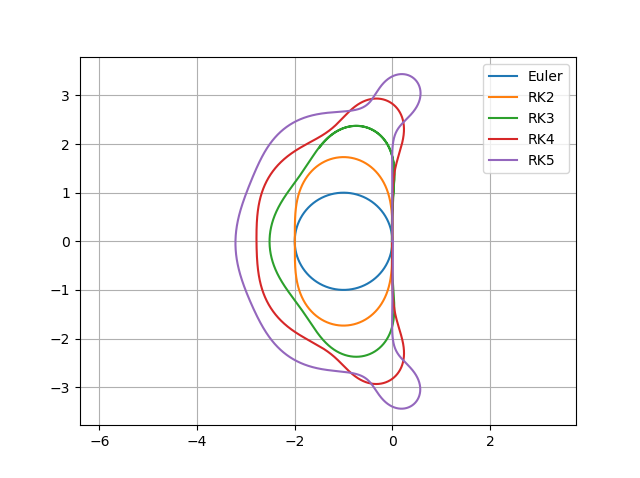
\includegraphics[width=0.5\textwidth]{imagenes/RK_explicitos.png}
    \caption*{Frontera de los dominios de estabilidad para los métodos RK explícitos de orden 1, 2, 3, 4 y 5.}
\end{figure}

\section{Estabilidad absoluta de los métodos multipasos}

\begin{defi}
    Se denomina polinomio de estabilidad absoluta del método multipaso
    \begin{align*}
        \sum_{i=0}^{q} \alpha_i y_{k+i} = h\sum_{i=0}^{q} \beta_i f_{k+i},
    \end{align*}
    al polinomio:
    \begin{align*}
        \Pi(z,\hat{h}) = \rho(z) - \hat{h}\sigma(z).
    \end{align*}
\end{defi}

\begin{obs}
    Podemos asegurar que todas las soluciones de la ecuación $y' = \lambda y$, $\text{Re}(\lambda) < 0$ tienden a 0 cuando $t \to \infty$ si y solo si todas las raíces de $\Pi(z;\hat{h})$ tienen módulo estrictamente menor que 1.
\end{obs}

\begin{defi}
    Se denomina dominio de estabilidad absoluta
    \begin{align*}
        D_A = \{ \hat{h} \in \mathbb{C} : \Pi(z;\hat{h}) = 0 \Longrightarrow|z| < 1\}.
    \end{align*}
\end{defi}

\begin{defi}
    Se denomina intervalo de estabilidad absoluta a $I_A = D_A \cap \mathbb{R}$.
\end{defi}

\begin{defi}
    Se dice que el método es $A-$estable si $\mathbb{C}^- \subset D_A$.
\end{defi}

\subsection{Método de localización de la frontera}
Definimos
\begin{align*}
    \partial D_A = \{ \hat{h} \in \mathbb{C} : \Pi(z;\hat{h}) \text{ tiene alguna raíz de módulo 1}\}.
\end{align*}
Es claro que $Fr(D_A) = \partial D_A$. Si $\hat{h} \in \partial D_A$, existe $\theta \in \mathbb{R}$ tal que $\Pi(e^{i\theta};\hat{h}) = 0$, es decir, existe $\theta \in \mathbb{R}$ tal que $\rho(e^{i\theta}) - \hat{h}\sigma(e^{i\theta}) = 0$, si $\sigma(e^{i\theta}) \not = 0$, entonces
\begin{align*}
    \hat{h} = \frac{\rho(e^{i\theta})}{\sigma(e^{i\theta})}.
\end{align*}
Consideramos en $\mathbb{C}$ la curva:
\begin{align*}
    \theta \in \mathbb{R} \ : \ \sigma(e^{i\theta}) \longmapsto \frac{\rho(e^{i\theta})}{\sigma(e^{i\theta})}.
\end{align*}
Esto nos da una curva que contiene a la frontera de $D_A$.

Aplicando este método a los métodos AB, AM y BDF:

\begin{figure}[H]
    \centering
    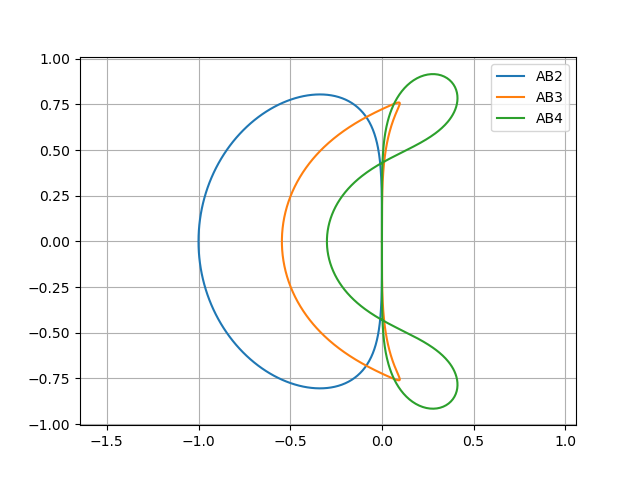
\includegraphics[width=0.5\textwidth]{imagenes/Metodos_AB.png}
    \caption*{Frontera de los dominios de estabilidad para los métodos AB de 2, 3 y 4 pasos.}
\end{figure}

\begin{figure}[H]
    \centering
    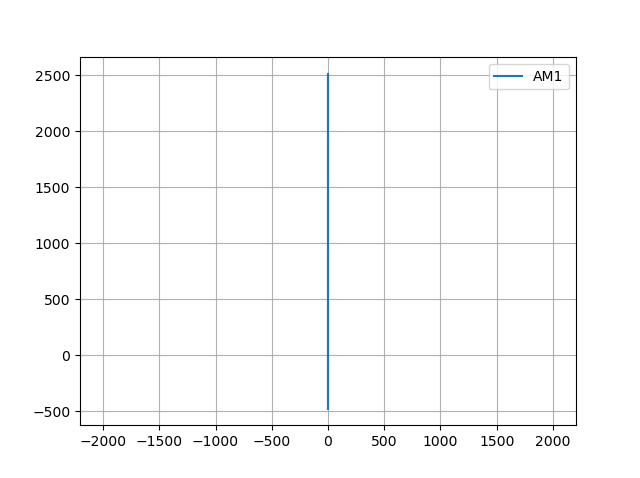
\includegraphics[width=0.5\linewidth]{imagenes/AM1.png}
    \caption*{Frontera del dominio de estabilidad del métodos AM1.}
\end{figure}


\begin{figure}[H]
    \centering
    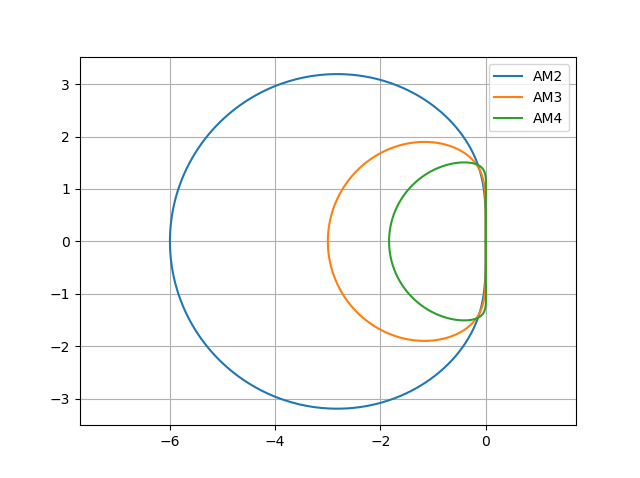
\includegraphics[width=0.5\linewidth]{imagenes/AM.png}
    \caption*{Frontera de los dominios de estabilidad para los métodos AM de 2, 3 y 4 pasos.}
\end{figure}

\begin{figure}[H]
    \centering
    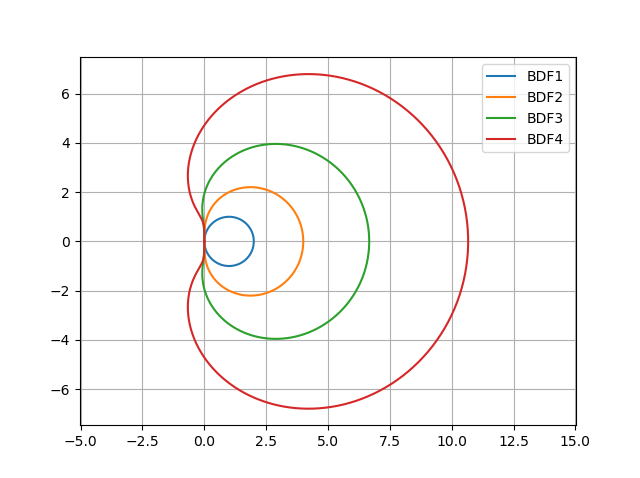
\includegraphics[width=0.5\textwidth]{imagenes/BDF.png}
    \caption*{Frontera de los dominios de estabilidad para los métodos BDF de 1, 2, 3 , 4 y 5 pasos.}
\end{figure}

\section{Otros tipos de ecuaciones con comportamiento Stiff}
Los problemas \textit{stiff} son aquellos que presentan ciertas características que hacen que sean difíciles de resolver utilizando métodos numéricos tradicionales. Estas características incluyen la presencia de términos que varían de forma muy rápida o muy lenta en el tiempo, o la presencia de términos que varían de forma muy rápida o muy lenta en el espacio. Estos términos pueden hacer que los métodos numéricos tradicionales tengan un rendimiento inaceptablemente lento o inestable. Veamos un ejemplo donde podamos observar estas características.

\begin{ejemplo} \
    \begin{enumerate}
        \item
              \begin{align*}
                  \left\{ \begin{array}{lcc}
                              y' = \lambda y, \ \ \text{Re}(\lambda) < 0 \\
                              y(0) = y_0                                 \\
                          \end{array}
                  \right.
              \end{align*}
        \item
              \begin{align*}
                  \left\{ \begin{array}{lcc}
                              \overrightarrow{y}' = M\overrightarrow{y}, \ \ \ A \in M_{N \times N} \\
                              \overrightarrow{y}(0) = \overrightarrow{y_0}
                          \end{array}
                  \right.
              \end{align*}
    \end{enumerate}
\end{ejemplo}

\section{Estabilidad absoluta de los métodos Predictor-Corrector}
Consideremos el método P-C que para cada $k = 0,1,\ldots$
\begin{align*}
    \left\{ \begin{array}{lcc}
                z_0 = y_k + hf(t_k,y_k)                               \\
                z_{l+1} = y_k + hf(t_{k+l},z_l), \ \ l = 0,\ldots,M-1 \\
                y_{k+1} = z_M
            \end{array}
    \right.
\end{align*}
Calculemos $R(\hat{h})$. Aplicamos el método P-C para resolver
\begin{align*}
    \left\{ \begin{array}{lcc}
                y' = \lambda y, \ \ \text{Re}(\lambda) < 0 \\
                y(0) = y_0                                 \\
            \end{array}
    \right.
\end{align*}
Una vez calculado $y_k$:
\begin{align*}
    z_0 & = y_k + h\lambda y_k = (1 + \hat{h})y_k                                                                \\
    z_1 & = y_k + h\lambda y_k = (1 + \hat{h})z_0 = y_k + \hat{h}(1 + \hat{h})y_k = (1 + \hat{h} + \hat{h}^2)y_k \\
    \vdots                                                                                                       \\
    z_M & = \ldots = (1 + \hat{h} + \ldots + \hat{h}^{M+1})y_k
\end{align*}
Con lo que tenemos que $y_{k+1} = z_M = (1 + \hat{h} + \ldots + \hat{h}^{M+1})y_k = (1 + \hat{h} + \ldots + \hat{h}^{M+1})^{k+1}y_0$, luego, $R(\hat{h}) = 1 + \hat{h} + \ldots + \hat{h}^{M+1}$.
\begin{itemize}
    \item Si $M = 0$, $R(\hat{h}) = 1 + \hat{h}$, que es la función de estabilidad del método de Euler.
    \item Si $M = \infty$, $R(\hat{h}) = 1 + \hat{h} + \hat{h}^2 + \ldots = \frac{1}{ 1- \hat{h}}$, que es la función de estabilidad del método de Euler implícito.
\end{itemize}
